\chapter[Dinámica de una partícula]{DINÁMICA DE UNA PARTÍCULA}\label{chap:cap2}
\startcontents
\printchaptertableofcontents

En el capítulo anterior examinamos el movimiento de una partícula desde una perspectiva puramente geométrica, es decir, describimos cómo se desplaza sin indagar en las causas que lo originan. Esta aproximación, conocida como cinemática, nos permitió caracterizar trayectorias, velocidades y aceleraciones en distintos sistemas de referencia.

En este capítulo damos un paso esencial: el estudio de las causas del movimiento. Ya no nos limitaremos a describir lo que ocurre, sino que buscaremos comprender por qué ocurre. Para ello, introduciremos el concepto de fuerza y analizaremos cómo influye sobre el comportamiento dinámico de los cuerpos. Este cambio de enfoque nos conduce al dominio de la dinámica, cuya base conceptual son las leyes formuladas por Isaac Newton en el siglo XVII.

La dinámica establece la relación entre el movimiento de un objeto y las fuerzas que actúan sobre él. Las leyes de Newton formalizan esta conexión y constituyen el núcleo de la mecánica clásica, proporcionando un marco general para predecir el comportamiento de sistemas físicos bajo diversas condiciones.

A lo largo del capítulo, estudiaremos estas leyes fundamentales y su aplicación al movimiento de partículas. También introduciremos nociones clave como la masa, la fuerza neta y los sistemas de referencia inerciales, herramientas esenciales para entender tanto los fenómenos cotidianos como los problemas más complejos de la física.

\section{Leyes de Newton}

\begin{definition}{Primera Ley de Newton}{primera_ley_newton}
    Todo cuerpo que esté en reposo o con movimiento rectilíneo uniforme, se mantendrá en reposo o con movimiento rectilíneo uniforme siempre que no exista agente externo que sobre el actúe
\end{definition}

Por agente externo entendemos una fuerza que se ejerza sobre el cuerpo. El texto tomado de la obra de Newton dice:
\begin{primera}
    Todo cuerpo persevera en su estado de reposo o movimiento uniforme y rectilíneo a no ser en tanto que sea obligado por fuerzas impresas a cambiar su estado.
\end{primera}

Galileo Galilei llamó inercia a la propiedad de los cuerpos de mantener su reposo o MRU. Los sistemas de referencia en donde se observa esta propiedad se llaman \textit{sistemas inerciales}.

\begin{definition}{Segunda Ley de Newton}{segunda_ley_newton}
    La fuerza neta que actúa sobre una partícula es igual al producto de su masa por su aceleración instantánea
    $$\F = m\acei.$$
\end{definition}

Entendemos por fuerza neta; la fuerza total, la suma de todas las fuerzas que actúan sobre la
partícula. Es decir,
$$\F = \sum_{i=1}^{N}\F_i.$$
Por otro lado,
$$m\acei = m \frac{d\veloi}{dt} = \frac{d\posi}{dt}$$
donde $\posi = m\veloi$ es un vector llamado \textit{cantidad lineal de movimiento} o \textit{momento lineal}. Es decir, la fuerza neta es la derivada \textit{(fluxión)} del momento lineal.
$$\F = \frac{d\posi}{dt}.$$
El texto toado de la obra de Newton dice:
\begin{segunda}
    El cambio de movimiento es proporcional a la fuerza motriz impresa y ocurre según la línea recta a lo largo de la cual aquella fuerza se imprime.
\end{segunda}

En su obra formal sobre los principios matemáticos de la física, Isaac Newton previo a sus axiomas o leyes del movimiento, da una serie de definiciones que vale la pena mostrar.
\begin{defpri}
    La cantidad de materia es la medida de la misma originada de su densidad y volumen conjuntamente.
    
    A esta cantidad llamo en lo sucesivo cuerpo o masa. Se hace manifiesta por el peso de cualquier cuerpo, pues, por medio de experimentos muy exactos con péndulos, hallé que era proporcional al peso.
\end{defpri}

\begin{defseg}
    La cantidad de movimiento es la medida del mismo obtenida de la velocidad y de la cantidad de materia conjuntamente.
\end{defseg}

\begin{defcua}
    La fuerza impresa es la acción ejercida sobre un cuerpo para cambiar su estado de reposo o movimiento uniforme y rectilíneo.
\end{defcua}

\begin{definition}{}{tercera_ley_newton}
    A toda fuerza de acción le corresponde otra de reacción de igual magnitud que actúa sobre la misma línea de acción, pero de sentido opuesto.
\end{definition}

Estas fuerzas de acción y de reacción siempre actúan en cuerpos distintos. El texto tomado de la obra de Newton dice:
\begin{tercera}
    Con toda acción ocurre siempre una reacción igual y contraria: O sea, las acciones mutuas de dos cuerpos siempre son iguales y dirigidas en direcciones opuestas.
\end{tercera}

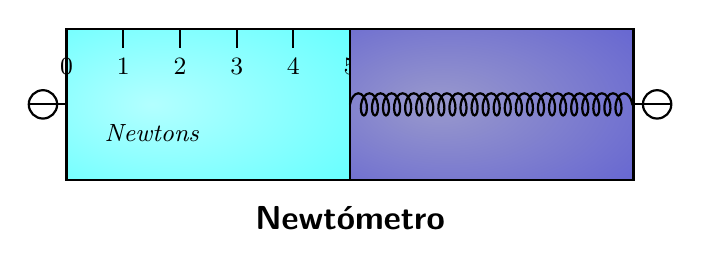
\begin{tikzpicture}[scale=1.2, every node/.style={font=\sffamily}]

% --- Definición de degradados ---
\pgfdeclareradialshading{azulclaro}{\pgfpoint{-10bp}{0bp}}%
  {color(0bp)=(cyan!30); color(40bp)=(cyan!60); color(80bp)=(cyan!30)}

\pgfdeclareradialshading{azuloscuro}{\pgfpoint{-10bp}{0bp}}%
  {color(0bp)=(blue!50!black!40); color(40bp)=(blue!70!black!60); color(80bp)=(blue!50!black!40)}

% --- Cuerpo izquierdo (escala) ---
\shade[shading=azulclaro] (-4,0.8) rectangle (-1, -0.8);
\draw[thick] (-4,0.8) rectangle (-1,-0.8);

% Escala de 0 a 5 N
\foreach \i in {0,...,5} {
  \draw[thick] (-4 + 0.6*\i,0.8) -- (-4 + 0.6*\i,0.6);
  \node[font=\small] at (-4 + 0.6*\i,0.4) {\i};
}
\node[font=\itshape\small, anchor=west] at (-3.7,-0.3) {Newtons};

% Gancho izquierdo
\draw[thick] (-4,0) -- (-4.4,0);
\draw[thick] (-4.4,0) arc (180:540:0.15);

% --- Cuerpo derecho (resorte) ---
\shade[shading=azuloscuro] (-1,0.8) rectangle (2, -0.8);
\draw[thick] (-1,0.8) rectangle (2,-0.8);

% Resorte
\draw[thick,decoration={coil,aspect=0.5,segment length=4pt,amplitude=4pt},decorate] 
     (-1,0) -- (2,0);

% Gancho derecho
\draw[thick] (2,0) -- (2.4,0);
\draw[thick] (2.4,0) arc (0:360:0.15);

% Título
\node[font=\sffamily\bfseries\large] at (-1,-1.2) {Newtómetro};

\end{tikzpicture}

\begin{semblanza}{Sir Isaac Newton}{1642–1727}[Newton.jpg]
    Sir Isaac Newton fue una de las mentes más brillantes y determinantes en la historia del pensamiento humano. Matemático, físico, astrónomo, alquimista, filósofo natural y teólogo inglés, su obra transformó de manera profunda y duradera la forma en que la humanidad concibe el universo. Nació el 25 de diciembre de 1642 (según el calendario juliano) en Woolsthorpe, Lincolnshire, en el seno de una Inglaterra convulsionada por intensos conflictos políticos y religiosos. Desde temprana edad manifestó una curiosidad inagotable y una capacidad excepcional para la observación y el razonamiento.

    Su obra capital, los \textit{Philosophi\ae\ Naturalis Principia Mathematica} (1687) —conocida comúnmente como los *Principia*— estableció los fundamentos de la mecánica clásica mediante la formulación de las tres leyes del movimiento y la ley de la gravitación universal. En un contexto todavía dominado por el pensamiento aristotélico y la escolástica, Newton demostró que el cosmos opera bajo leyes matemáticas precisas, comprensibles y universales. Con ello, no sólo consolidó una nueva visión racional del universo, sino que sentó las bases del método científico moderno.

    Su genio se extendió mucho más allá de la física. Fue, junto con Leibniz, uno de los creadores del cálculo infinitesimal, desarrollado de forma paralela e independiente. En el ámbito de la óptica, demostró que la luz blanca está compuesta por una gama de colores, estableciendo los cimientos de la teoría moderna del color. Asimismo, diseñó el primer telescopio reflector funcional, conocido hoy como telescopio newtoniano, una innovación que revolucionó la observación astronómica.

    Hombre de pensamiento profundo y religiosidad intensa, Newton dedicó gran parte de su vida a la alquimia y al estudio meticuloso de las Escrituras. Aunque estas facetas fueron objeto de escepticismo por parte de sus contemporáneos y de generaciones posteriores, revelan su convicción de que todo conocimiento —científico, espiritual o simbólico— forma parte de una misma verdad universal aún por desvelar.

    Fue miembro de la Royal Society, institución que presidió durante más de dos décadas, y ocupó el cargo de director de la Casa de la Moneda del Reino Unido, donde desempeñó un papel clave en la reforma del sistema monetario. En 1705, fue nombrado caballero por la reina Ana, pasando a ser reconocido como Sir Isaac Newton.

    Falleció el 20 de marzo de 1727 y fue sepultado con honores en la Abadía de Westminster, privilegio reservado a las grandes figuras de la nación. Su epitafio, aunque tácito, pervive en la memoria colectiva de la humanidad:
    \begin{center}
        \textit{“Si he visto más lejos, es porque estoy sentado sobre los hombros de gigantes.”}
    \end{center}
    Una frase que él mismo escribió y que resume, con humildad, la grandeza de su legado.

    Newton no sólo revolucionó la ciencia, transformó radicalmente nuestra concepción de la realidad. Su influencia es tan vasta que, siglos después, sus ideas siguen constituyendo pilares fundamentales de la formación científica. Su pensamiento riguroso, su creatividad sin límites y su incansable búsqueda del conocimiento continúan inspirando a quienes anhelan comprender las leyes que rigen el universo.
\end{semblanza}

% \section{Leyes de Fuerzas}

% \section[Ley de Gravitación Universal]{Ley de Gravitación Universal de Newton}

% \section{Ley de Coulomb}

% \cleardoublepage